\chapter{Introduction}

\graphicspath{ {report/Chapter1/assets/} } 

\section{Project Overview}

The core objective of this MSc dissertation project is to assist in the development of an ultra low-cost wearable EEG (electroencephalogram) sensor prototype being developed by Imperial's NGNI (Next Generation Neural Interfaces) for demonstration at the Royal Society Summer Science Exhibition 2021. 

\section{Scope and Objectives}
To develop real time decoding and subsequent visualisation of raw analogue EEG signals acquired from proprietary EEG hardware devices developed by the NGNI lab. As these devices will be worn by up to 100 people during the Royal Society Exhibition, EEG decoding and visualisation needs to happen simultaneously to enable a virtual multiplayer game controlled by participating members of the audience.

\section{Constraints}
The task of using this device at scale in a public setting imposes some unique practical constraints. These are outlined below:
\begin{itemize}
    \item production at scale: 100+ replicas of the EEG device need to be produced.
    \item very tight budget of $\approx$ £20 per device.
    \item hardware must be self-contained and so all computation should happen on the hardware. 
    \item there is to be minimal calibration required from the user. If any, it should be done automatically.
    \item real time decoding and feedback of signals (or as close to real time as possible).
    \item user needs to be able to receive feedback on decoded signals - ideally visually.
    \item device should be unobtrusive and cannot use `wet' electrodes that would hamper the user experience.
\end{itemize}

Furthermore, the EEG hardware in development is based on the low-cost Espressif ESP32 SoC based on the Tensilica Xtensa LX6 MCU. Features that are relevant to this specific project include: 
\begin{itemize}
    \item dual-core, 240MHz CPU
    \item onboard FPU
    \item up to 600 DMIPS performance
    \item ultra low-power (ULP) co-processor
    \item 4 MiB SRAM
    \item integrated WiFi 802.11 b/g/n and BLE
\end{itemize}
Fortunately, the ESP32 SoC is extremely capable for its low cost (less than £5) and should be sufficient to handle on board computation for DSP and decoding provided that it is implemented efficiently. Its dual-core feature is also particularly useful as it will allow computation and networking to run concurrently. 

\subsection{Constraint implications}
The constraints listed above have substantial implications on my project. One of the largest constraints is the budget of £20; entry level consumer-grade BCIs (brain computer interfaces) typically cost in the region of $\$100-\$1000$. As a result, our device will only have \textbf{two active EEG channels}. Although most BCIs have many more active channels, many studies have shown that a viable decoding system can be achieved with only a limited number of channels \cite{Wang2011}, some with even as few as 2 \cite{Acampora2021}. 

The prohibition of wet electrodes is also significant. Wet electrodes are known to significantly improve the quality\footnote{by reducing contact impedance} of the electrical connection to the scalp which would invariably improve SNR. 

The number of samples required for adequate frequency resolution is an important consideration. Initial analysis in the experiments outlined below showed that around 5 seconds worth of sampling at 256Hz was required to achieve adequate frequency resolution. Consequently, computation time is unlikely to be the limiting factor in achieving real time decoding.

% \section{Skills Areas}
% This project will require the following core skills areas: 
% \begin{itemize}
%     \item signal processing
%     \item machine learning and/or pattern recognition
%     \item embedded programming of a microcontroller
%     \item visualisation using a web app interface and some basic client-server infrastructure
% \end{itemize}

\section{Proposed EEG Analysis Strategy}
As alluded to before, one of the objectives for the Royal Society Exhibition is to create a multiplayer game that receives control signals from participants in the audience wearing our EEG devices. Thus, one of the responsibilities of this project is to decide on the specific EEG paradigm that will be used to capture user input. It should be noted that the feasibility of various paradigms largely depends on the quality of the available signals and that of the decoding pipeline which are yet to be conclusively determined. Several studies suggest that \textbf{steady-state visual evoked potentials} \cite{Fernandez-Fraga2016}\cite{Kanoga2020}\cite{Acampora2021} (SSVEPs) offer significant potential for EEG decoding tasks similar to this project due to the high information transfer rate (ITR), non-invasiveness and relatively high SNR that can be achieved using basic BCI devices \cite{Zhu2021}. 
\subsection{SSVEP decoding}

\begin{wrapfigure}{r}{0.2\textwidth} %this figure will be at the 
\vspace{-1cm}
    \centering
    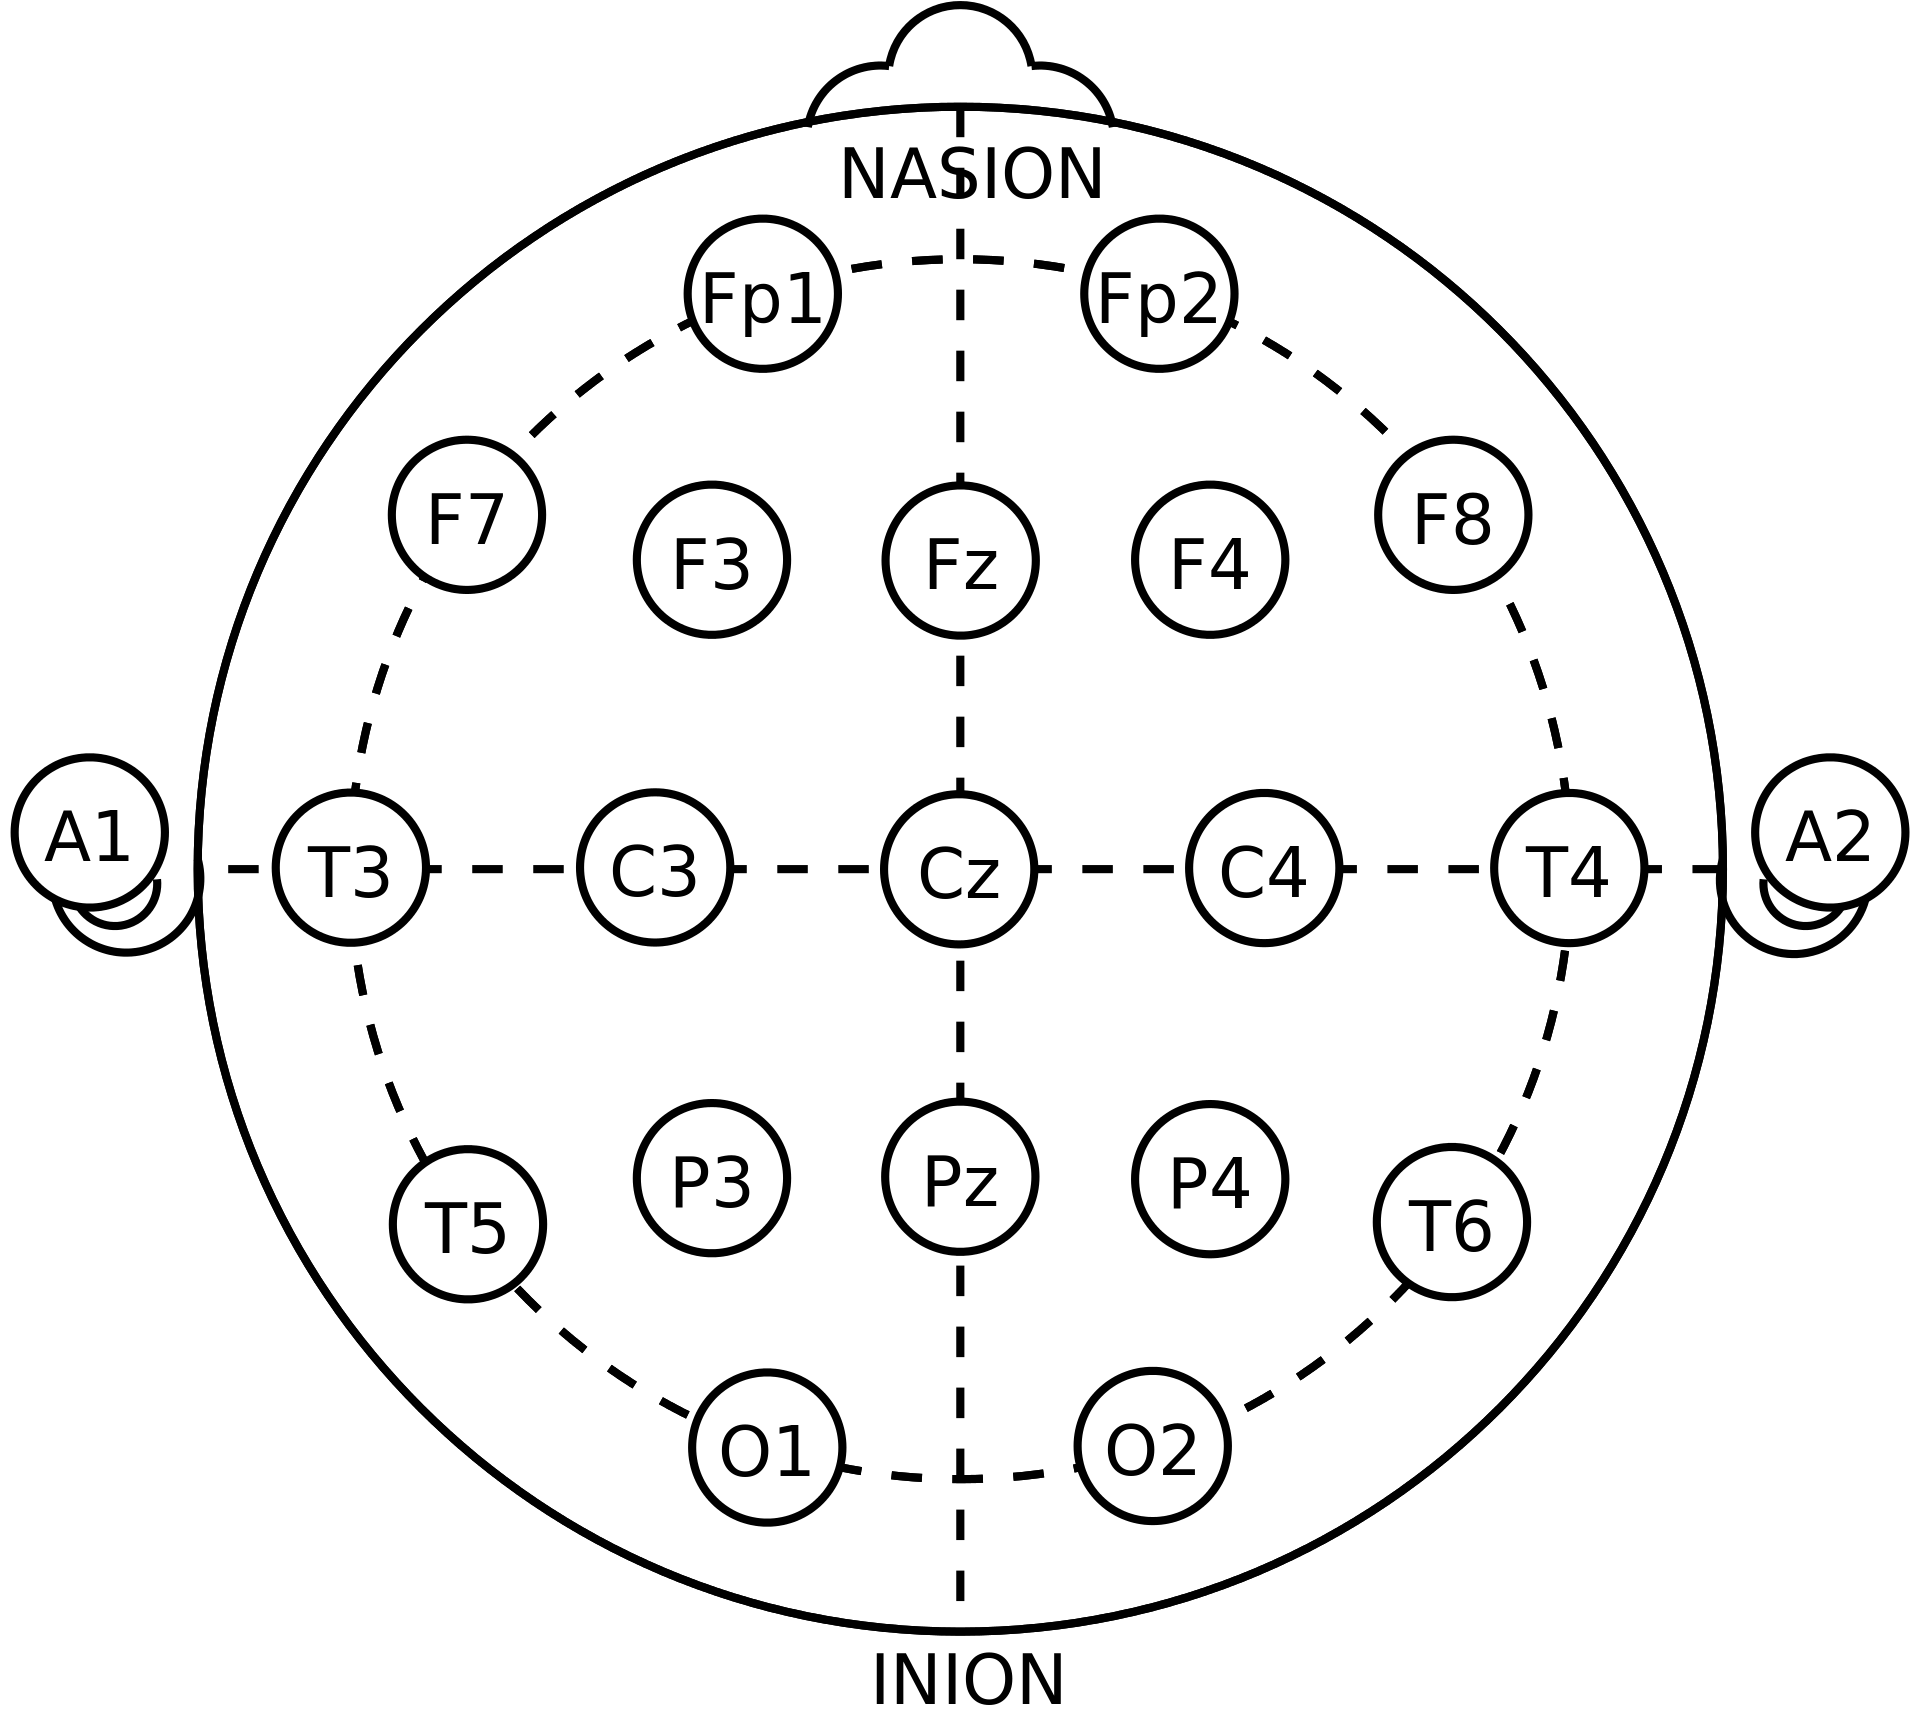
\includegraphics[height=1.2in]{10-20.png}
    \caption{10-20 electrode scheme}
    \label{fig:c1-10-20}
\end{wrapfigure}

An SSVEP signal is most commonly observed as the brain's response to a visual stimulus flickering at constant frequency \cite{Xie2016}. Specifically, the fundamental SSVEP frequency $f_{SSVEP}^{(0)}$ will match that of the stimulus in the spectrum of the resulting EEG signal (within some frequency bounds, as explored below). Stimulus frequency bands of around 8-15Hz are commonly used \cite{Acampora2021}\cite{Chen2017}, however, Xie et al showed successful decoding with 27.8Hz \cite{Xie2016}. SSVEPs are produced in the brain's visual cortex and are usually measured in the occipital and/or parietal regions \cite{Fernandez-Fraga2016}. Using the international 10-20 electrode electrode scheme, this corresponds to the $\text{PO}_x$ and $\text{O}_x$  electrodes. The current idea is that users in the exhibition will be presented a mobile-friendly, lightweight web page with 2-4 stimulus squares or other images that flicker at frequencies $f_1, \dots, f_n$. Each stimulus will correspond to an action - such as `up' or `down' - that will control an avatar in the cooperative game mentioned above. The objective is to decode $f_1, \dots, f_n$ in order to interpret a user's desired action (i.e. discern which stimulus image they are focused on).

\section{Preliminary Experiments and Next Steps}
At the time of writing, several preliminary experiments have been conducted to assess the feasibility of the proposed EEG decoding schemes under the aforementioned constraints. An SSVEP dataset  was extracted from the study in \cite{Acampora2021} that used limited EEG channels and a low-cost data acquisition system, as will be the case in this project. Preliminary frequency domain analysis showed promising results; using Welch periodograms computed using STFTs (short-term Fourier transforms), frequency spikes could be distinguished at frequencies corresponding to those of the stimuli as documented in the study.

Towards generating our own data under conditions that are comparable to those anticipated in the final product, experimentation has begun on an OpenBCI EEG kit\footnote{available online from \href{https://shop.openbci.com/products/bundle2?variant=13036379766856}{OpenBCI Inc.}}. A data acquisition and analysis interface has been implemented in python and is successfully able to stream, store and process data from the device. Furthermore, an ESP32 SoC board has been purchased and set up. In order to assess feasibility of on-device computation, an efficient FFT algorithm has been implemented on the MCU and seems effective: thanks to its FPU, single precision, 1024 length FFTs can be executed in under 1ms. All software under development is being managed with version control and can be accessed \href{https://github.com/JamesTev/EEG-decoding}{here}.



% \begin{table}[]
% \centering
% \label{tab:c1-eeg-paradigms}
% \begin{tabular}{@{}lll@{}}
% \toprule
% \textbf{EEG Paradigm} & \textbf{Description} & \textbf{Tentative Feasibility} \\ \midrule
% ERP                   & \begin{tabular}[c]{@{}l@{}}Event-related potentials are measurable responses to specific\\ sensory, cognitive or motor events. The P300 wave measured in\\ the oddball experiment represents a signal deflection in response\\ to an `odd' or uncommon target stimulus in between common \\ non-target stimuli.\end{tabular} & more feasible                  \\
% SSVEP                 & \begin{tabular}[c]{@{}l@{}}Steady state visually-evoked potentials are responses to visual \\ stimuli at specific frequencies\end{tabular}                                                                                                                                                                                   & more feasible                  \\
% MI                    & Motor imagery                                                                                                                                                                                                                                                                                                                & less feasible                 
% \end{tabular}
% \caption{Comparison of common EEG paradigms under consideration}

% \end{table}
\clearpage

\section{Preliminary Experimental Figures}
Figure \ref{fig:psd-1} below shows spectral estimates using a standard periodogram and a Welch-averaged periodogram. The power peak at $f=15$Hz corresponds to the SSVEP stimulus frequency of $f_*=15$Hz in the experiment from \cite{Acampora2021}. The EEG signal of 16s in length was sampled at $f_s=256$Hz and an FFT length of $N=1024$ samples was used. A Hanning window length of $\Delta n=N$ was used. The Welch periodogram used 50\% overlap for window averaging.
\begin{figure}[h]
\centering
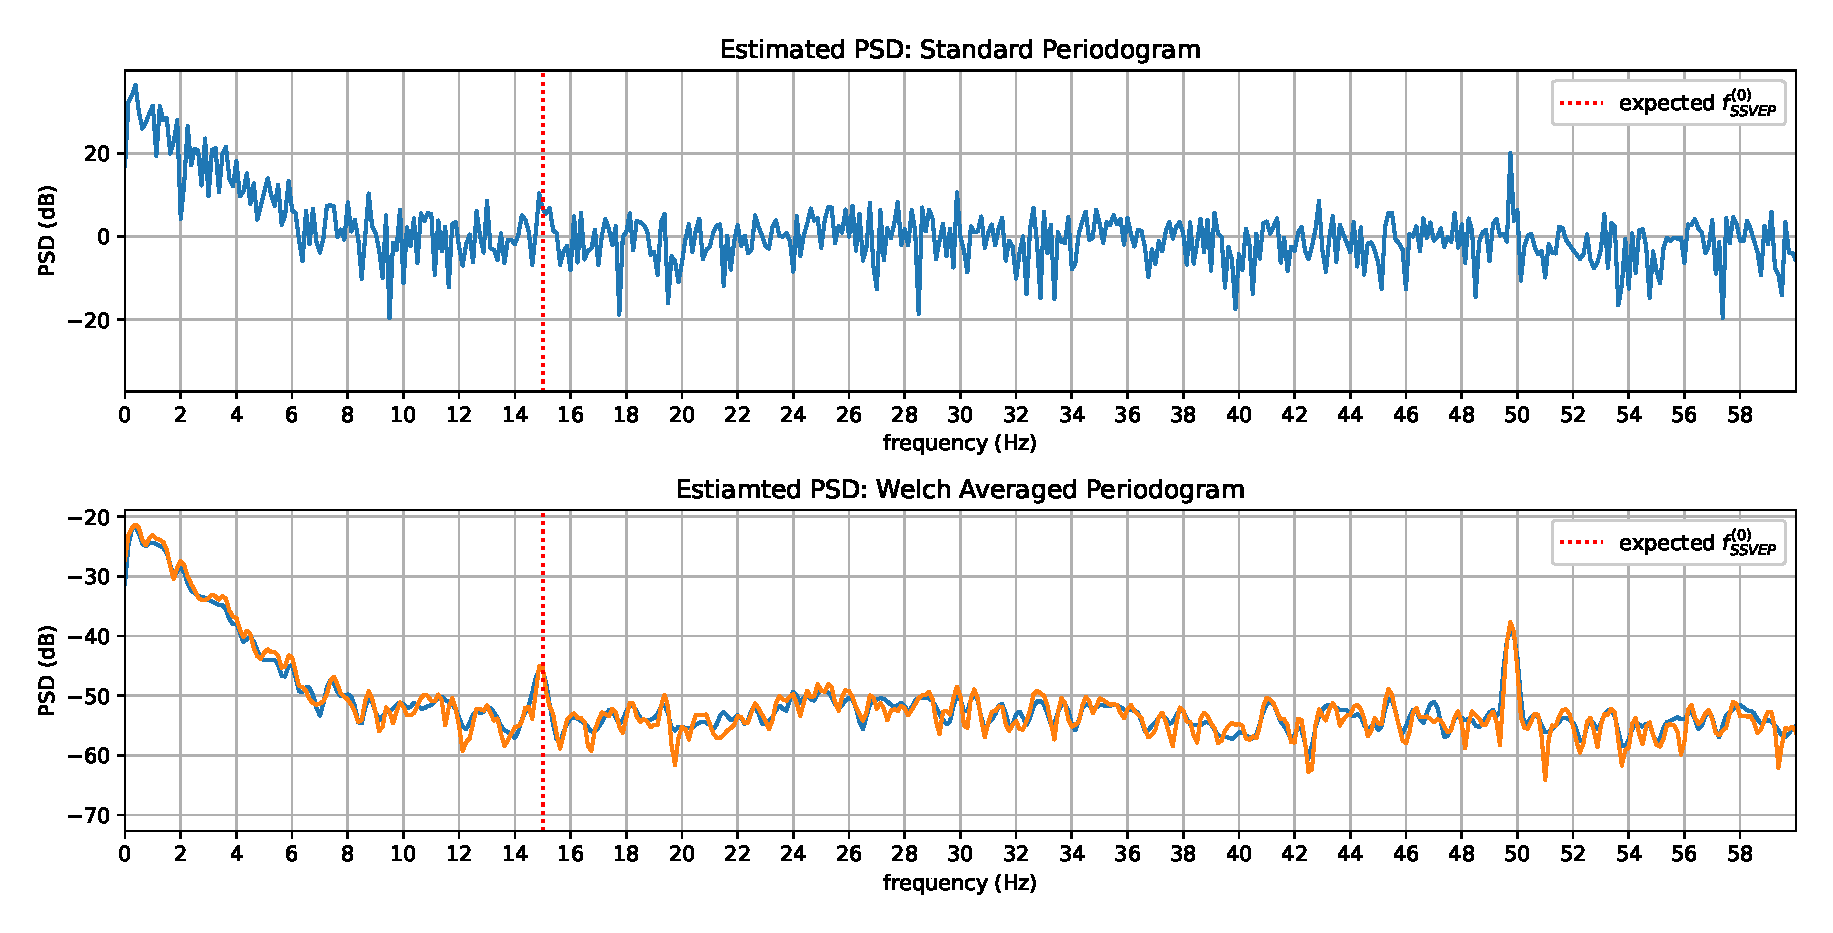
\includegraphics[width=\textwidth]{psd_plot}
\caption{Power spectral density estimates of a single channel EEG signal in response to a stimulus frequency of $f_*=15$Hz}
\label{fig:psd-1}
\end{figure}
